\documentclass[12pt]{article}
\usepackage{graphicx, caption, subcaption}
\captionsetup[figure]{font=small}

% Page margins
\usepackage[a4paper, total={6.5in, 8.8in}]{geometry}

% Indentation
\usepackage{indentfirst}
\setlength{\parindent}{2em}
\setlength{\parskip}{1em}

% Page numbering
\usepackage[utf8]{inputenc}
\usepackage[english]{babel}
\usepackage{fancyhdr}
\usepackage{lastpage}
 
\pagestyle{fancy}
\fancyhf{} % sets both header and footer to nothing
\renewcommand{\headrulewidth}{0pt} % no top line
\cfoot{Page \thepage \hspace{1pt} of \pageref{LastPage}}

% Random options
\captionsetup{font=Large}
\graphicspath{ {./images/} }

% Tables
\usepackage{booktabs}


%------------------------------------------------------------

\begin{document}

\begin{titlepage}
    \centering
    {\Large
        Instituto Superior Técnico --- Taguspark\par
        Network and Computer Security\par
    }
    \vfill
    
    {\Huge\bfseries
        Smartphone as a security token\par (Proposal)\par
    }
    \vspace{6ex}
    {\Large
        Group 18\par
    }
    \vfill
    
    \begin{figure}[h!]
    \centering
        \begin{subfigure}{.5\textwidth}
        \centering
        \captionsetup{justification=centering}
            
\includegraphics{ist173891}
            \caption*{
                ist173891 --- David Gonçalves\par
                david.s.goncalves@tecnico.ulisboa.pt
            }
        \end{subfigure}%
        \begin{subfigure}{.5\textwidth}
        \centering
        \captionsetup{justification=centering}
            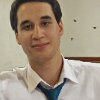
\includegraphics{ist194104}
            \caption*{
                ist194104 --- Leonardo Troeira\par
                leonardo.troeira@tecnico.ulisboa.pt
            }
        \end{subfigure}\vspace{6ex}
        
        \begin{subfigure}{1\textwidth}
        \centering
        \captionsetup{justification=centering}
            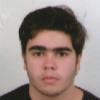
\includegraphics{ist194122}
            \caption*{
                ist194122 --- Francisco do Carmo\par
                francisco.baptista.carmo@tecnico.ulisboa.pt
            }
        \end{subfigure}
    \end{figure}
    
\end{titlepage}
    
%------------------------------------------------------------

\newpage

\section{Problem}
    
Password-based authentication has the advantage of being simple and convenient to use. However, there are too many attacks that can be performed remotely that render this authentication mechanism not secure enough on its own---phishing, XSS, SQLI, rainbow tables, dictionary attacks, brute force... to name a few.\par

As such, if we're seeking stronger security mechanisms, one option is to make use of multi-factor authentication, usually involving knowledge and possession. This poses a trade-off between security and usability however, since the user will be needing to carry something with him all the time (e.g. smartphone).\par

Besides authentication mechanisms, we're also faced with the challenge of data possibly being stolen, either by sniffing network packets or acquiring control over the victim's file system, among other possible attacks. Therefore, assuring that data is stored and transmitted securely (relying on encryption algorithms) is a must. And again, for additional security, we should have another factor of authentication.\par

\subsection{Requirements}

\begin{enumerate}
  \item The web server must have mechanisms to prevent XSS and SQLI.
  \item Communication between client and server must be done through a custom secure channel.
  \item The system must provide two-factor authentication.
  \item User files must be stored encrypted.
  \item User files must be decrypted only if the user has their smartphone nearby the client application.
  \item The system must provide fault tolerance. If the system crashes after decrypting the files, make sure that the files are encrypted again.
  \item Communication between the smartphone and client application must be done using a secure protocol.
  
\end{enumerate}

\subsection{Trust assumptions}

Our problem assumes that the network and user's device cannot be trusted. However, we assume that the user's device is not compromised while it is in use, and that the smartphone and server are not compromised either. We also assume that the server's certificate is trusted.

%------------------------------------------------------------

\newpage
\section{Proposed solution}

For our solution, we shall create a simple website---on a server machine---with a register and login forms, for which we shall obviously sanitize user input and make use of SQL parameters in order to prevent XSS and SQLI respectively. The user's password shall be stored hashed and salted in order to prevent it from being easily obtained by potential attackers. As an additional security layer for authentication, we shall use 2FA with the help of Duo SDK, thus leveraging the smartphone's proximity to the user as part of an increased security solution. The server shall also log any user actions.\par

The user shall be able to download files, from the server's website, which come encrypted with a symmetric key. The user's key pair shall be generated at the registration phase, and they shall be stored in the user's smartphone, which will necessarily need to be connected to the user's device in order to be able to receive it, and we shall make a simple Android app for this purpose. The smartphone and user's device shall connect through Wi-Fi, utilizing a secure protocol (e.g. WPA2/3). For extra security, the user's private key should be symmetrically encrypted with a password, which should be different than the user's login password (e.g. KeyStore). The symmetric key used for each file shall also be stored in the smartphone encrypted in the same fashion as the user's private key.\par

We shall create a simple client application for viewing these encrypted files that were downloaded from the server. In order for the client application to decrypt these files, the smartphone must be connected to the user's device. The system shall be fault tolerant---as soon as this connection is lost, the client application shall clean its state, thus the user shall no longer be able to view the encrypted files. We plan on using a stream cipher for this purpose, as in theory we can have large files that don't fit in volatile memory.\par

For registration and login, an AES key shall be exchanged using a secure protocol (e.g. Diffie-Hellman). Subsequent communication between the user and the server shall be done using symmetric encryption with this key, in order to guarantee confidentiality. For integrity, each message shall be hashed together with random padding (using SHA-2) and for authenticity this hash shall be signed with the sender's private key.\par

%------------------------------------------------------------

\setcounter{figure}{0} % Reset figure counter
\begin{figure}
\centering
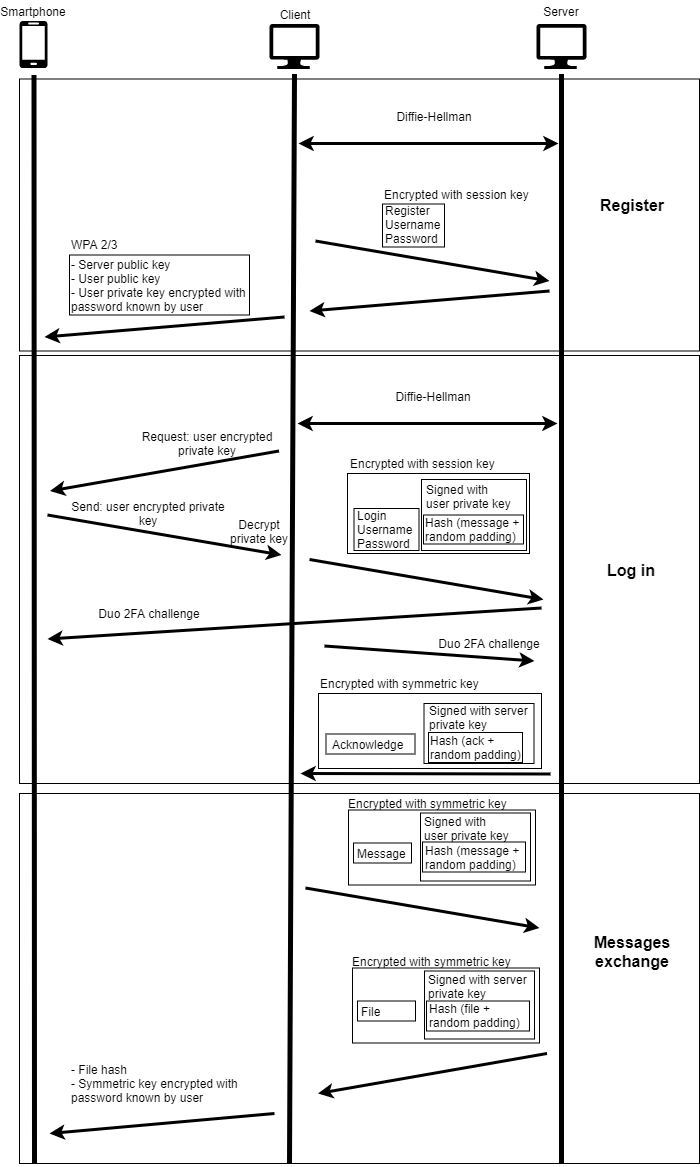
\includegraphics[width=12cm]{secure_channel_2.png}
\caption{Secure communication}
\end{figure}

%------------------------------------------------------------

\newpage
\section{Plan}

\subsection{Versions}

\begin{itemize}
  \item \textbf{Basic:} For our basic solution we shall create a website with a register and a login forms, with mechanisms to prevent XSS and SQLI attacks, that stores passwords hashed and salted, creates a key-pair for each user upon registration and gives it to them. The server shall also be able to encrypt trivial text files---context doesn't matter---with a symmetric key shared with the user at login, and allow the user to download them.  We shall then create a simple client application (typically JavaScript on the website) so that these files can be viewed by the user, using a stream cipher.

  \item \textbf{Intermediate:} On top of the basic version, we shall implement 2FA using Duo SDK and add another use for our smartphone, which is proximity detection. The user's key pair, server public key and symmetric key for each file shall be stored in the smartphone, we'll design a simple Android app to take care of this task. The communication with the smartphone shall use a secure Wi-Fi protocol (WPA 2 or 3). We shall also log user actions on the server side.

  \item \textbf{Advanced:} Finally, to complete our solution, we shall guarantee that as soon as the connection to the smartphone is lost or the client application crashes, the encrypted files shall no longer be visible. Additionally, we'll design our own custom secure channel for communication between server and client, as explained in the previous chapter. We'll also encrypt the user's private key and files' symmetric keys using an AES key derived from a password that only the user knows about.
\end{itemize}

\subsection{Effort commitments}

% https://www.tablesgenerator.com/#
\begin{table}[h]
\footnotesize
\begin{tabular}{@{}p{1cm}|p{4cm}|p{4cm}|p{4cm}|@{}}
\cmidrule(l){2-4}
 & 73891 - David Gonçalves & 94104 - Leonardo Troeira & 94122 - Francisco Carmo \\ \midrule
\multicolumn{1}{|l|}{4 Nov - 10 Nov} & Create Server/Client Sides & Create Android App & Create Server/Client sides \\ \midrule
\multicolumn{1}{|l|}{11 Nov - 17 Nov} & Create secure channel between server and client & Configure 2FA with Duo SDK & Create secure channel between server and client \\ \midrule
\multicolumn{1}{|l|}{18 Nov - 24 Nov} & Add security to data with cryptography & Add security to data with cryptography & Configure standard secure channel between smartphone and server \\ \midrule
\multicolumn{1}{|l|}{25 Nov - 1 Dec} & Add fault tolerance to server & Add fault tolerance to server & Add fault tolerance to server \\ \midrule
\multicolumn{1}{|l|}{2 Dec - 8 Dec} & Test System/Correct bugs & Test System/Correct bugs & Test System/Correct bugs \\ \midrule
\multicolumn{1}{|l|}{9 Dec - 11 Dec 17H} & Write Report & Write Report & Write Report \\ \bottomrule
\end{tabular}
\end{table}

%\begin{figure}[ht]
%\centering
%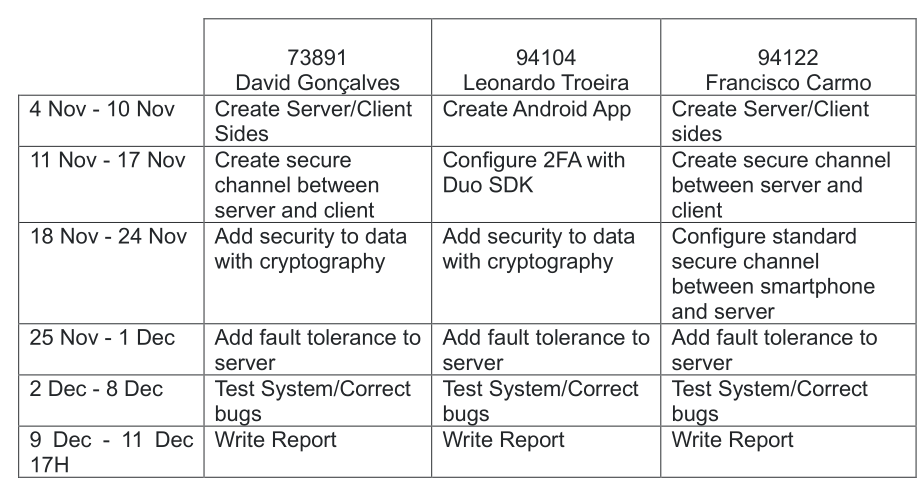
\includegraphics[width=15cm]{plan}
%\end{figure}

%------------------------------------------------------------

\newpage
\section{References}

\begin{itemize}
  \item \textbf{Duo SDK:} Duo's trusted access solution is a user-centric zero-trust security platform to protect access to sensitive data at scale for all users, all devices and all applications.\par https://duo.com/product/every-application/supported-applications/apis\par
  Found: Yes\par
  Installed: No\par
  Tested: No\par
\end{itemize}

\end{document}